\documentclass[color]{tudbook}
\usepackage{tudthesis, german}
\usepackage[utf8]{inputenc}
\usepackage{bibgerm}


\begin{document}
\einrichtung{Fakult"at Elektrotechnik und Informationstechnik,}
\institut{Institut f"ur Automatisierungstechnik}
\thesis{Dokumentation zum Projekt Mensch-Maschine-Systemtechnik}
\author{Gruppe 6: Dominik Baumann, Johannes Börnicke, Katrin Messbauer, Angela Wobar}
\title{Weiterentwicklung einer Revisionsdarstellung für das Revisionsverwaltungssystem R43ples}
\supervisor{Dipl.-Ing. M. Graube}
\submitdate{05. Februar 2016}
\maketitle

\tableofcontents

\chapter{Motivation}
Um mit mehreren Personen koordiniert an großen Softwareprojekten arbeiten zu können, ist ein Versionsverwaltungssystem unerlässlich. Insbesondere für das Semantic Web mangelt es derzeit noch an einem solchen System, weshalb es in der Industrie noch nicht akzeptiert ist. Das Semantic Web stellt eine Erweiterung des Webs dar, mit der Informationen einfacher austausch- und verwertbar werden sollen, indem zu Begriffen zusätzliche semantische Informationen hinzugefügt werden. In \cite{Graube} wird mit \textit{R43ples} ein Konzept für ein solches Versionsverwaltungssystem vorgestellt. Zur Visualisierung werden hier gerichtete Graphen verwendet. In der vorliegenden Arbeit soll die vorhandene Visualisierung erweitert werden, um die Changesets, der einzelnen Revisionen sichtbar zu machen. Dabei werden zunächst bestehende Konventionen und Ästhetikkriterien für Graphen untersucht und die bisherigen Arbeiten an R43ples, sowie andere Konzepte für Versionsverwaltungssystemen für das Semantic Web bzw. Linked Data im Allgemeinen analysiert werden, um auf dieser Basis anschließend eine eigene Visualisierung zu entwerfen und zu implementieren.

\chapter{Stand der Technik}
In \cite{Gruppe2.3,Gruppe2.1} wurden bereits Visualisierungen für Das Revisionsverwaltungssystem R43ples entwickelt. Diese sollen im Folgenden analysiert werden, nachdem zunächst einige allgemeine Richtlinien für das Erstellen von Visualisierungen von Graphen dargelegt wurden. Anschließend werden noch weitere Visualisierungen von Linked Data aus der Literatur diskutiert.

\section{Grundlegende Richtlinen}
\label{sec:Richtlinien}
Ein Graph ist definiert als eine Menge an Knoten und Kanten, wobei jede Kanten zwei Knoten aus dieser Menge verbindet \cite[Seite 2]{Graphenoptimierung}. Sie dienen zur Veranschaulichung von Relationen zwischen Objekten und können dabei u.a. in gerichtete und ungerichtete Graphen unterteilt werden. Bei ungerichteten Graphen wird nicht zwischen Start- und Zielknoten unterscheiden, bei gerichteten Graphen ist eine solche Unterscheidung vorhanden \cite{diskreteMathematik}. Für die Aufgabenstellung liegt also ein gerichteter Graph vor, da jeder Knoten einen Vorgänger und einen Nachfolger hat und diese klar unterscheidbar sind.

Für das Zeichnen von Graphen existieren einige Konventionen, die z.B. in \cite{Aesthetik} aufgeführt sind. Hier soll die Konvention, dass alle Kanten als gerade Linie gezeichnet werden sollen, eingehalten werden. Zudem soll auf eine planare Zeichnung geachtet werden, was bedeutet, dass sich Kanten höchstens an Knoten schneiden sollen. Neben den Konventionen gibt es einige Ästhetikkriterien, die ebenfalls bestmöglich umgesetzt werden sollen. Dazu zählt die Minimierung der Schnittpunkte von Kanten, der Fläche und der Gesamtkantenlänge.

\section{Bisherige Visualisierungen}
In \cite{Gruppe2.1} ist eine Möglichkeit zur Visualisierung bereits dargestellt. In diesem Entwurf steht der Graph im Mittelpunkt. Die einzelnen Knoten sind mit der Revisionsnummer beschriftet und durch die Pfeile ist ersichtlich, wie der Verlauf der Branches ist. Gleiche Branches sind zudem durch gleiche Farben gekennzeichnet. Durch einen Haken können zusätzlich die Tags angezeigt werden. In einem mouseover Feld werden bei Bedarf weitere Informationen angezeigt. Die Commits sind von unten nach oben angeordnet. Hierbei ist aber die zeitliche Abfolge der Commits in unterschiedlichen Branches nicht ersichtlich.

Die zweite Visualisierung in \cite{Gruppe2.3} stellt den Graphen mehr an die Seite und stellt mit Kommentar zu jedem Commit sowie dem Autor zusätzliche Informationen dar. Die zeitliche Abfolge ist hier ersichtlich, zu dem ist eine Einteilung in Monate gegeben. Der Graph wird durch diese Darstellung allerdings relativ klein und der Text dominiert die Visualisierung.   

\section{Weitere Literatur}
\label{sec:WeitereLiteratur}
In \cite{Git2PROV} wird mit W3C PROV ein neuer Standard eingeführt, um Versionskontrollsysteme wie Git einfacher benutzen und veröffentlichen zu können, vgl. Abb. \ref{fig:Git2PROV}. Dort sind viele Informationen des semantischen Netzes dargestellt, durch verschiedene Formen getrennt. Damit ist das Format weniger intuitiv und es braucht eine gewisse Einarbeitungszeit, bis damit umgegangen werden kann. Dieses Modell ist eher als Werkzeug für Entwickler gedacht und damit als Vorlage für R43ples nicht geeignet, da hier mehr auf den Anwender eingegangen werden soll, der die wesentlichen Informationen dargestellt haben möchte anstatt einer ausführlichen Beschreibung des semantischen Netzes.

\begin{figure}[htbp] 
  \centering
     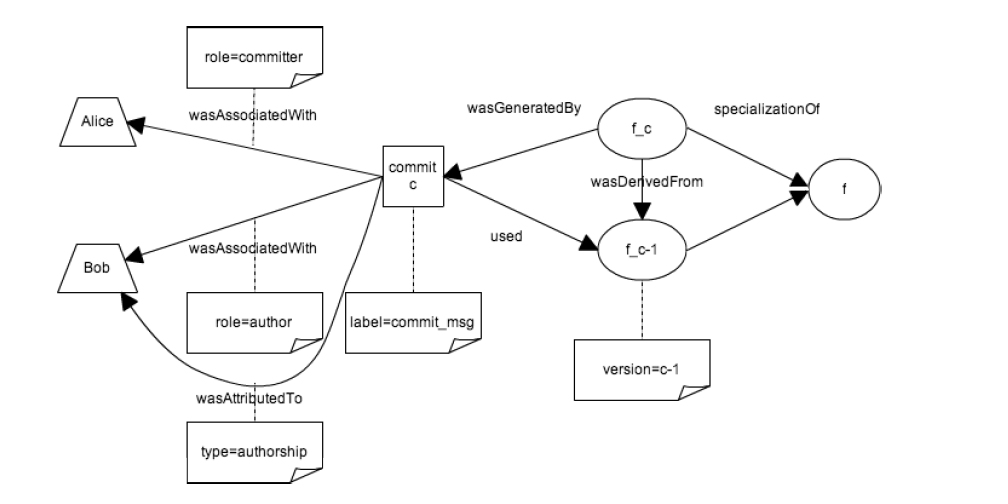
\includegraphics[width=\textwidth]{Git2PROV.png}
  \caption{Darstellung eines Graphen mit Git2PROV}
  \label{fig:Git2PROV}
\end{figure}

\chapter{Anforderungsdefinition}
Ideen:
\begin{itemize}
\item Mouseover für mehr Informationen
\item Evtl. durch Klick dauerhaftes Hinzufügen der Informationen
\item Show und Hide Haken
\item evtl Änderung der Form auf Rechteck, um mehr Platz für zusätzliche Informationen zu erhalten
\item Commits und Tags sollen weiterhin klar unterscheidbar sein, evtl. durch Farbe
\item Vermeiden von Kreuzungen
\item Ausgleich zwischen Information und Übersichtlichkeit finden
\item Neuestes nach oben
\item Evtl. Master in der Mitte, alles andere drum herum anordnen
\item Evtl. Einfügen einer Suche
\item Entscheidendes Ziel der zusätzlichen Informationen: Schnelles Finden der Version, die wiederhergestellt werden soll
\item add und remove durch Symbol darstellen
\item Mit Klick/Mouseover Informationen, was geaddet bzw. removed wurde
\item Sortierung nach Datum? Evtl. auch grobe Zeiteinteilung
\end{itemize}

\section{Einleitung}
\subsection{Zielsetzung}
In der vorliegenden Arbeit soll die im vorangegangenen Abschnitt analysierte, vorhandene Visualisierung für das semantische Revisionsverwaltungssystem R43ples erweitert werden, sodass die Inhalte der Changesets der Revisionen sichtbar werden. Der neue Entwurf soll sich dabei gut in die bisherige HTML-Oberfläche integrieren und gut skalieren in Bezug auf die Größe der Changesets.

\subsection{Produktziele}
Die Entwicklung soll als Fork auf GitHub durchgeführt werden, als Implementierungssprache ist Javascript vorgesehen. Es existiert eine HTML-Oberfläche, die weiter verwendet werden soll.

\section{Allgemeine Beschreibung}
\subsection{Produktumgebung}
Revisionsverwaltungssysteme werden im Allgemeinen vorwiegend auf Desktop-PCs oder Laptops verwendet, evtl. auch auf Tablets. Deshalb ist es sinnvoll, von einem Bildschirm im Querformat auszugehen. Deshalb soll der Graph, statt wie in der bisherigen Visualisierung, anstatt von oben nach unten von links nach rechts angezeigt werden, um den Platz optimal auszunutzen und so auch lange Graphen ohne Scrollen darstellen zu können.

\subsection{Benutzereigenschaften}
Anders als die in Abschnitt \ref{sec:WeitereLiteratur} beschriebene Visualisierung, die eher für Entwickler gedacht ist, ist R43ples für Anwender gedacht, die keine ausführliche Darstellung des semantischen Netzes, sondern eine übersichtliche Visualisierung der wichtigen Informationen benötigen. 

\subsection{Produktfunktion}
\begin{enumerate}
\item Übersichtlichkeit und Lesbarkeit der Graphen durch Einhalten der Richtlinien und Kriterien aus Abschnitt \ref{sec:Richtlinien}, sowie durch Beschränken auf die entscheidenden Informationen
\item Automatische Anordnung der Revisionen nach Zeitpunkt des Commits und der Verbindungen
\item Hervorheben des Master Branches, kennzeichnen der Branches mit Namen und Gruppierung durch einheitliche Farbgebung
\item Direkt dargestellt werden soll zudem die Revisionsnummer
\item Hinzufügen weiterer Informationen wie Changeset oder Kommentar durch Mouseover bzw. Klicken
\end{enumerate}

\subsection{Allgemeine Einschränkungen und Randbedingungen}



\chapter{Umsetzung}

\bibliography{MMST}
\bibliographystyle{gerabbrv}

\end{document}
